\chapter{Introduction}\label{chpt:intro}

\section{Motivation}\label{sec:intro/motivation}
Ever since the first digital audio workstations were introduced in the early
1990s, the audio waveform has been the primary method of navigating audio
content. The waveform works well for finding amplitude-related events such as
silences and peaks, but is very poor at conveying much more about the sound of
the content. Additionally, the waveform doesn't scale well as demonstrated by
the `Soundcloud sausage' (see Figure~\ref{fig:soundcloud}), where even at
reasonable zoom levels, no useful information is presented.  A popular
alternative to the waveform is the spectrogram, which displays detailed
information about the frequency content. However, these can be very difficult
to interpret and require training and practice to be of use.

\begin{figure}[ht]
  \centering
  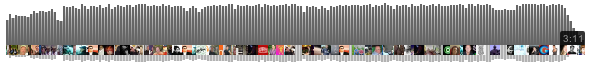
\includegraphics[width=0.6\textwidth]{figs/soundcloud.png}
  \caption{An example of a waveform visualization on the online music sharing
    service Soundcloud}
  \label{fig:soundcloud}
\end{figure}

\section{Aim}\label{sec:intro/aim}
This projects aims to develop better visualization for helping radio producers
navigate audio content by initially targeting a number of common tasks. Audio
features will be identified or developed which are able to capture the
information required for the task. Methods of mapping these features to an
image will be created so that the information is presented in a perceptible way
which requires little or no training. 

\section{Thesis structure}\label{sec:intro/structure}

\paragraph{Section \ref{sec:litreview}} reviews existing work and literature
from three areas that will feed into the project -- feature extraction,
visualization and cross-modal links.

\paragraph{Section \ref{sec:production}} provides a comprehensive overview of
the radio production process at the BBC, which will help put this research into
context.

\paragraph{Section \ref{sec:study}} details the process and results of an
initial online study which looked at how the waveform performs in a common
production tasks, and whether it can be improved.

\paragraph{Section \ref{sec:tech}} considers the technical developments made in
the project so far.

\paragraph{Section \ref{sec:plan}} outlines a research plan for the rest of the
project, including a discussion of potential opportunities for novel
contributions and a timetable for completion.

\section{Contributions}\label{sec:intro/contributions}

\section{Associated publications}\label{sec:intro/publications}
